\begin{figure}[t]
\centering       
    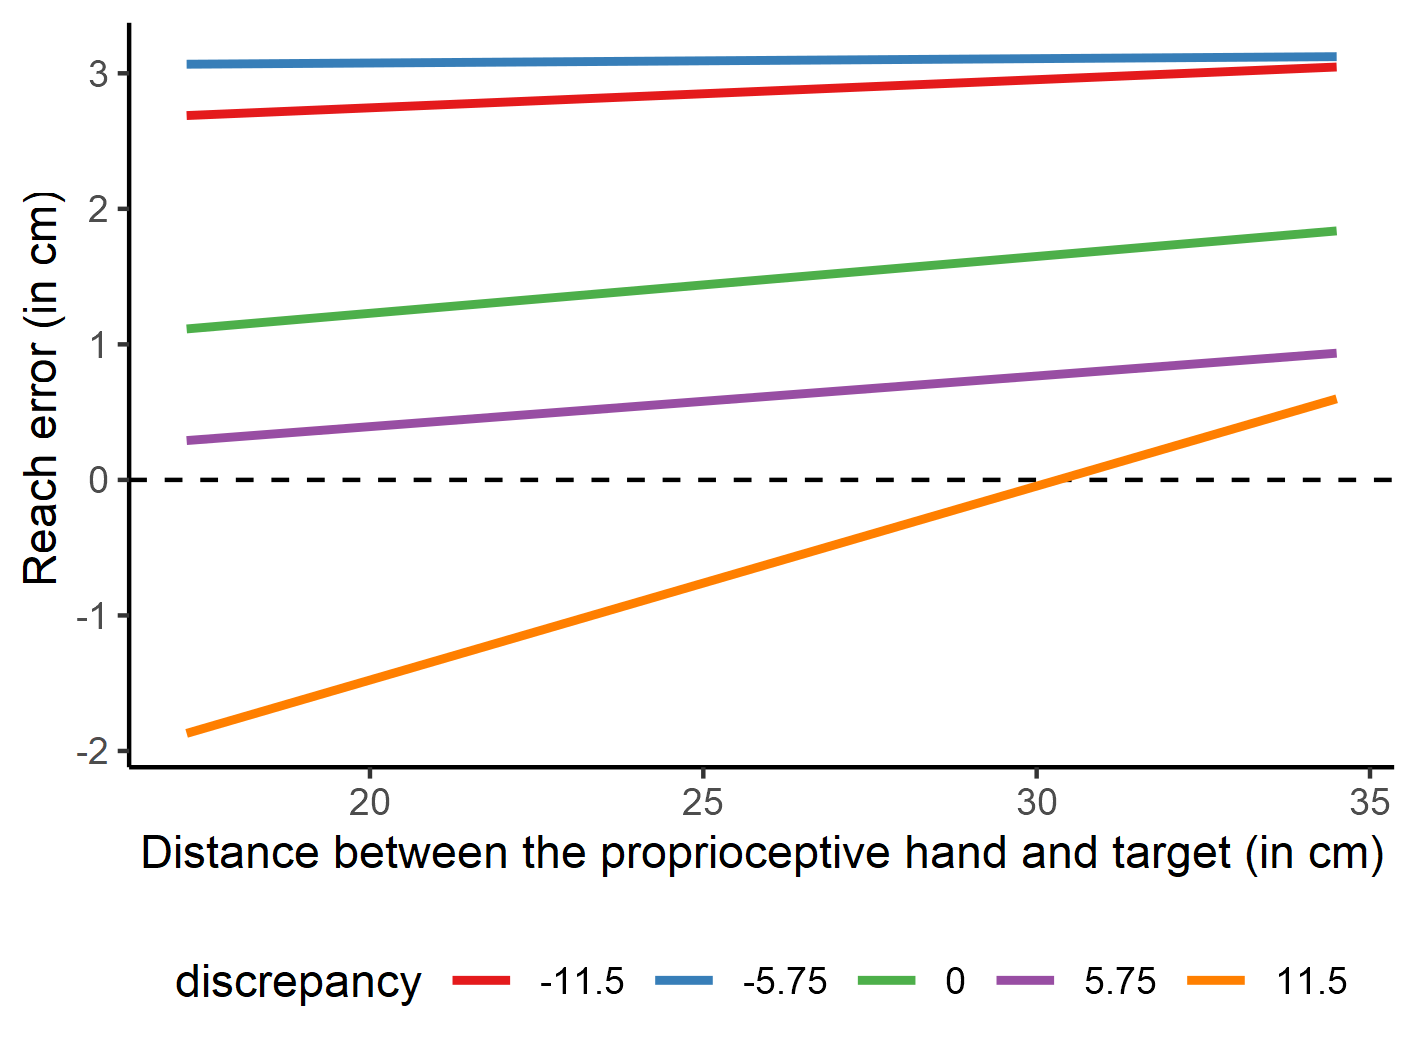
\includegraphics[scale=0.8]{Images/exp2_results.png}
    \caption{Reach error as a function of spatial discrepancy between the position of visual hand and the position of actual (proprioceptive) non-action hand. Each panel shows the distance between the target and the initial position of the action hand (AHT). Negative reach error indicates that the estimation of the target location was in the direction of the non-action hand towards the left, while positive reach error indicates that the location of the target was estimated in the direction of action hand towards the right of the actual location of the target.}
    \label{fig:exp2_re-pht}
\end{figure}